\chapter{Marco teórico}

\section{Manipulador robótico}

\subsection{Características Scorbot ER VII}

El Scorbot-ER VII es un  manipulador robótico de cinco grados de libertad (5 DOF) diseñado para propósitos educacionales. Posee la configuración estándar de robot industrial antropomórfico (Figura \ref{cap2_scorbot}), ie. \textit{base}, \textit{shoulder} y \textit{elbow}.

\begin{figure}[ht]
  \centering
  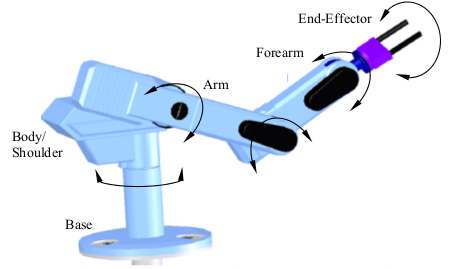
\includegraphics[scale=0.5]{img/cap2/scorbot}
  \caption{Scorbot-ER VII.}
  \label{cap2_scorbot}
\end{figure}

El sistema de actuación del robot se basa en el uso de poleas reductoras seguidas de engranajes armónicos (\textit{harmonic drives}) actuados por motores de corriente continua de imanes permanentes de una corriente máxima de \SI{18}{\ampere} a \SI{24}{\volt}. La carga máxima que puede llevar el robot es de \SI{2}{\kilo\gram} (incluido el peso del efector). Esta configuración asegura que el sistema es relativamente seguro para operar fuera de una jaula de seguridad \cite{scorbot1998}.

\section{Conceptos de cinemática}

Una de las tareas principales de un robot manipulador corresponde a seguir una trayectoria dejando al efector en una posición deseada. En orden de mover el robot a través de dos o más puntos de una trayectoria objetivo en un tiempo, velocidad y aceleración especificados, es necesario definir el movimiento de cada uno de los componentes del robot.

El análisis cinemático es el estudio del movimiento de los distintos elementos del robot, sin considerar las fuerzas y momentos que producen tal movimiento de los elementos.

\subsection{Cinemática directa}

Cinemática directa es el nombre que recibe el problema de encontrar la posición y orientación del efector relativo a la base del robot dados todas posiciones de las articulaciones y parámetros geométricos de los elementos que constituyen el robot. Usualmente, el sistema de referencia fijo en el efector se denomina \textit{tool frame} \cite{handbook}.

En la práctica, la cinemática directa es resuelta notando que para una cadena de elementos en serie, como es el caso del robot Scorbot, la transformada entre el sistema de referencia y el sistema fijo en el efector esta dada por la concatenación de las transformadas entre elementos adyacentes de la cadena cinemática.

\begin{equation}
T_0^5(\vec{\theta}) = T_0^1 T_1^2 T_2^3 T_3^4 T_4^5 
\end{equation}

Donde $\vec{\theta}=[\theta_1,\dotsc,\theta_5]$, $\theta_i$ corresponde al ángulo de la articulación $i$-ésima y $T_j^i$ es la transformada homogénea del elemento $i$ con respecto al sistema de referencia $j$.

\subsection{Cinemática inversa}

Por otro lado, la cinemática inversa es el nombre que recibe el problema de encontrar el valor de las posiciones de las articulaciones dada la posición y orientación del efector.
Usualmente, el cálculo de la cinemática inversa involucra la resolución de sistemas geométricos complejos que dificulta la obtención de formas cerradas, en casos donde la forma cerrada no existe se pueden emplear métodos numéricos basados en el jacobiano del sistema.

La obtención de modelos exactos de cinemática directa e inversa es tratado de forma extensa en \cite{cole2007} y \cite{predescu2015}.

\section{Motores de corriente continua}

El motor de corriente continua (CC) es la máquina eléctrica empleada en aplicaciones de potencia y tracción. Su sencillo principio de funcionamiento y gran versatilidad han permitido que siga vigente hasta nuestros días, a pesar de ser constructivamente más complejo que las que motores BLDC. Su velocidad fácilmente controlable, posibilidad de girar en ambos sentidos, lo hacen ideal para aplicaciones de tracción y control de posición.

El funcionamiento del motor de CC se basa en la fuerza generada por la interacción de un campo magnético inmóvil y uno generado por una bobina móvil, montada sobre un eje de rotación. La bobina móvil es alimentada a través de un sistema de escobillas y delgas para invertir la dirección de la corriente y, por consiguiente, el sentido del campo magnético generado, logrando que el torque resultante sea siempre favorable al sentido de giro \cite{vargas2006}. En la Figura \ref{cap2_motorcc} se muestra la bobina dentro de un campo magnético fijo de dirección horizontal.

\begin{figure}[H]
    \centering
    \begin{subfigure}[b]{0.4\textwidth}
            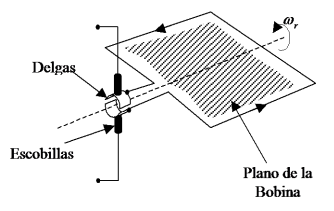
\includegraphics[width=\textwidth]{img/cap2/motor_cc1.png}
            \caption{Bobina elemental del motor de C.C. dispuesta sobre un eje de giro y alimentada a través de las escobillas.}
    \end{subfigure}%
    ~
    \begin{subfigure}[b]{0.4\textwidth}
            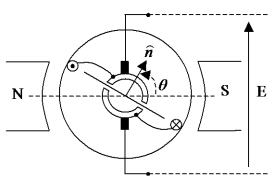
\includegraphics[width=\textwidth]{img/cap2/motor_cc2.png}
            \caption{Bobina montada en un rotor dentro de un campo magnético fijo cuya dirección es perpendicular al eje de giro.}
    \end{subfigure}
    \caption{Bobinas del motor CC}
    \label{cap2_motorcc}
\end{figure}



El circuito equivalente del motor CC se divide en dos partes: el circuito de excitación, que genera el campo magnético inmóvil; y el circuito motriz, en el que se representa al rotor (o armadura) como una fuente de tensión $E_a$. El campo magnético de dirección fija generado por el estator puede ser producido por imanes permanentes, como es el caso del los motores que posee el manipulador Scorbot ER-VII. La interacción entre ambos circuitos queda descrita por las siguientes ecuaciones:

\begin{eqnarray}
e_a &=& G \, \omega_r \, i_c \\
t &=& G \, i_{\phi} \, i_c
\end{eqnarray}

Donde Ea es el voltaje de armadura, $G$ es un parámetro de la máquina llamado inductancia rotacional, $\omega_r$ es la velocidad de giro del rotor y $t$ es el torque generado. Finalmente $i_{\phi}$ e $i_a$ son las corrientes de excitación y de armadura, respectivamente. Dado que se utilizan motores de imanes permanentes, por lo que el término $i_{\phi}$ se considera constante.

\subsection{Control de motores de corriente continua}

Para el control de motores de CC se utiliza un circuito llamado convertidor de puente completo o puente H, el cual utiliza la modulación de ancho de pulso (PWM) en una estructura de puente que permite la conducción en ambos sentidos, tal como se muestra en la Figura \ref{cap2_punteh}.

\begin{figure}[ht]
  \centering
  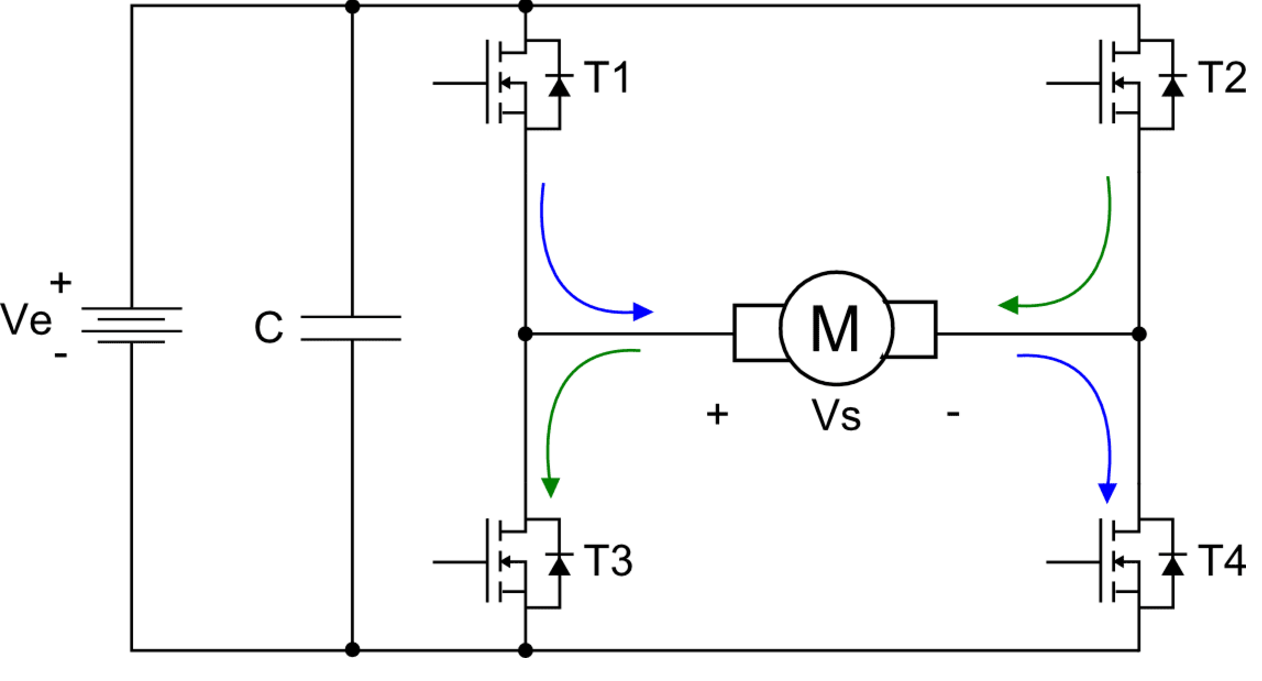
\includegraphics[scale=.2]{img/cap2/puenteh}
  \caption{Configuración del puente H.}
  \label{cap2_punteh}
\end{figure}

El uso de modulación PWM en el encendido de los transistores permite controlar la alimentación del motor CC. El diseño de estos dispositivos de potencia es un trabajo complejo, pues requiere la correcta elección de semiconductores, un \textit{layout} capaz de soportar altas corrientes y evitar la aparición de corrientes parásitas. Afortunadamente, dado la gran demanda de estos dispositivos por parte de la industria automovilística, fabricantes de semiconductores entregan soluciones acorde a los requerimientos. La Figura \ref{cap2_punteh_infineon} muestra un puente H fabricado por Infineon Technologies AG, que además de provee protección sobre sobrevoltaje y sobrecorriente.

\begin{figure}[ht]
  \centering
  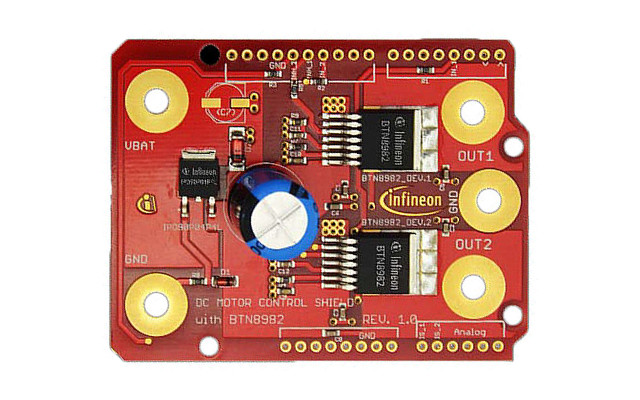
\includegraphics[scale=.35]{img/cap2/puenteh_infineon}
  \caption{Puente H fabricado por Infineon Technologies AG basado en BTN8982TA.}
  \label{cap2_punteh_infineon}
\end{figure}

\section{Interfaces hápticas}

Los dispositivos hápticos son capaces de proporcionar una retroalimentación de fuerza al usuario que lo emplea, de esta forma, complementan sistemas de operación visuales al entregar más información al operador. Esta tecnología puede aplicarse a múltiples sectores con el fin de facilitar su ejecución: medicina, realidad virtual, modelado, robótica, entre otras.

\subsection{Phantom Omni}

Phantom Omni es un dispositivo háptico de seis grados de libertad (6 DOF) desarrollado por Sensable, permite leer la posición de sus seis articulaciones y posee tres actuadores conectados a los tres primeras articulaciones, permitiendo la aplicación de fuerzas, que solo pueden controlar la posición del \textit{stylus} en el espacio cartesiano.

\begin{figure}[ht]
  \centering
  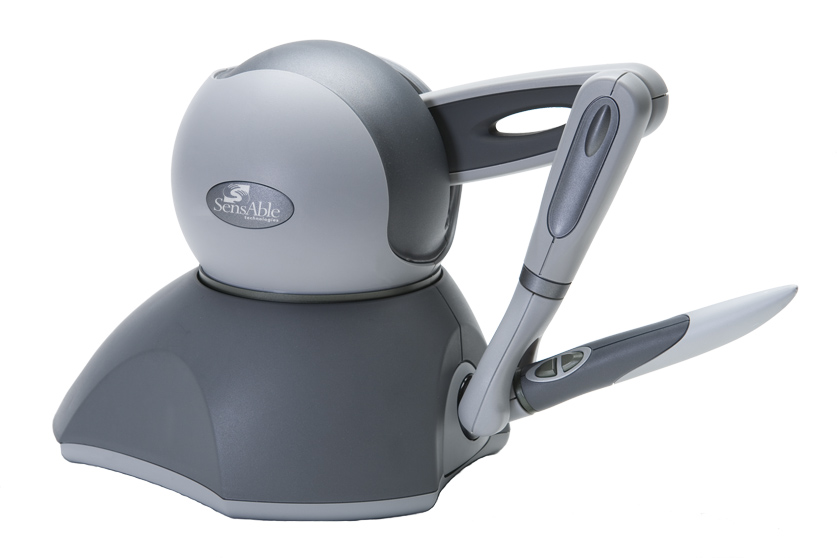
\includegraphics[scale=.2]{img/cap2/phantom_omni}
  \caption{Phantom Omni.}
  \label{cap2_phantom}
\end{figure}

Un aspecto importante del diseño es el desacople entre la posición y orientación \cite{beckman2007}, las tres primeras articulaciones son usadas para posicionar el \textit{stylus} y las restantes establecen la orientación del mismo. Los ejes de giro de estas últimas tres articulaciones se intersectan en un mismo punto, por lo que se puede interpretar como una articulación esférica.


\section{Componentes de software}

\subsection{ROS}

Robot Operating System (ROS) \cite{quigley2009} es un  framework para el desarrollo de aplicaciones robóticas, ofrece herramientas, librerías, abstracción de hardware, controladores de dispositivos, visualizadores, comunicación entre procesos, gestión de paquetes, entre otros.

A pesar de su nombre, ROS no es un sistema operativo propiamente dicho, es más bien un middlewere que se integra en sistemas GNU/Linux como Ubuntu. Una de sus principales ventajas es su amplia comunidad y que se encuentra bajo la licencia BSD, que permite el uso del software en aplicaciones comerciales. Fue desarrollado en 2007 por el Laboratorio de Inteligencia Artificial de Stanford bajo el nombre de \textit{switchyard}, luego su desarrollo continuó en el laboratorio de investigación robótico Willow Garage, actualmente la OSRF (\textit{Open Source Robotics Foundation}) es la encargada de mantener las herramientas básicas de ROS.

Uno es los aspectos más importantes de ROS es interfaz para la comunicación entre procesos. Un nodo, unidad de software básica en ROS, puede publicar o suscribirse a un tópico. En este tópico se escriben/leen mensajes que han sido depositados por otros nodos. Puede haber varios publicadores y subscriptores sobre el mismo tópico concurrentemente. Un único nodo puede publicar y subscribiese a múltiples tópicos.

Los mensajes son estructuras de datos que soportan tipos primitivos como
enteros, punto flotante, arreglos de primitivas y constantes. Adicionalmente los mensajes pueden estar compuestos por otros mensajes y por arreglos de mensajes, dando la profundidad que se requiera.

Otro elemento primordial lo constituyen los servicios, estos se definen mediante un par de mensajes, unos para la solicitud (\textit{request}) y otro para la respuesta (\textit{response}). Un nodo ofrece un servicio bajo un nombre y un cliente llama al servicio enviando un mensaje de solicitud y esperando a la respuesta.
